\section{Développements logiciel: Conception, Modélisation, Implémentation} 
\subsection{Description des modules utilisés}
% présenter les développements logiciels réalisés dans le cadre du projet
Pour la réalisation de ce projet, nous avons développé une application web qui permet de jouer
aux jeux du Hex et de l'Awalé avec la possibilité d'ajouter facilement d'autres jeux combinatoires. Ce logiciel est
composé de plusieurs modules, dont les principaux sont les suivants:

% présenter les principaux modules du logiciel développé dans le cadre du projet
% Utiliser le langage UML pour la modélisation : donner le diagramme de cas
% d'utilisation et le diagramme des classes
\begin{itemize}
    \item \textbf{Module Hex:} Ce module contient les classes et les fonctions nécessaires
    pour jouer au jeu du Hex. Il contient notamment la classe \texttt{HexBoard} qui 
    représente le plateau de jeu et les joueurs du jeu de Hex. Ce module contient également 
    les fonctions pour l'implémentation de l'algorithme \emph{MinMax} avec élagage alpha-bêta pour 
    la résolution du Hex.
    
    \item \textbf{Module Awalé:} Ce module contient les classes et les fonctions nécessaires
    pour jouer au jeu de l'Awalé. Il contient la classe \texttt{AwaleBoard} qui représente le
    plateau de jeu et les joueurs du jeu de l'Awalé. Ce module contient également les fonctions
    pour l'implémentation de l'algorithme \emph{MinMax} pour la résolution du jeu de l'Awalé. (À noter que la fonction \emph{MinMax}
    est la même pour les 2 jeux. Seul les fonctions d'évaluation changent.)
    
    \item \textbf{Module Interface Graphique:} Ce module contient les fichiers HTML, CSS et
    JavaScript nécessaires pour l'implémentation de l'interface graphique des jeux du Hex et
    de l'Awalé. Il contient notamment les fichiers \texttt{home.html}, \texttt{hex.html} et
    \texttt{awale.html} qui permettent à l'utilisateur de choisir le jeu auquel il veut jouer
    et les paramètres de la partie. Il contient également des fichiers JavaScript pour la
    gestion des événements et des intéractions avec l'utilisateur.
    
    \item \textbf{Module Test:} Ce module contient les fichiers de tests unitaires pour les
    classes et les fonctions des modules Hex et Awalé. Il contient notamment les fichiers
    \texttt{test\_hex.py} et \texttt{test\_awale.py}, qui permettent de tester les classes
    et les fonctions des modules Hex et Awalé. Il n'a été que partiellement implémenté 
    initiallement avant d'être mis de côté pour se concentrer sur d'autres aspects du projet.
\end{itemize}


% décrire les fonctionnalités de l'interface graphique implémentée (si votre 
% logiciel dispose d'une interface graphique)
\subsubsection{Fonctionnalités de l'interface graphique}
L'interface graphique de notre logiciel comprend une page d'accueil qui permet à l'utilisateur
de choisir le jeu auquel il souhaite jouer (Hex ou Awalé) et une page principale (home) pour chacun des jeux.
Cela permet à l'utilisateur de choisir les paramètres de la partie, comme la taille du plateau ou le 
mode de jeu. La page home permet aussi de consulter les règles du jeu sélectionné.
Lorsque l'on clique sur le bouton correspondant au mode de jeu choisi, nous sommes dirigés vers la page de
jeu.
Sur les deux jeux, le joueur à la possibilité de prévisualiser le prochain coup grâce à des fonctions de ``hover'' lorsqu'il survole avec 
la souris certains éléments.
Lors d'une partie de Hex, il est possible de changer le thème graphique avec la touche `H'. Cela modifie la page CSS chargée dans le navigateur.
L'interface graphique est implémentée en HTML, CSS et JavaScript. Celle-ci communique avec les modules Hex et Awalé via des appels de fonctions JavaScript à des
fonctions Python au travers de requêtes json et du module Flask.

\begin{figure}[!htb]
    \begin{minipage}{0.33\textwidth}
        \centering
        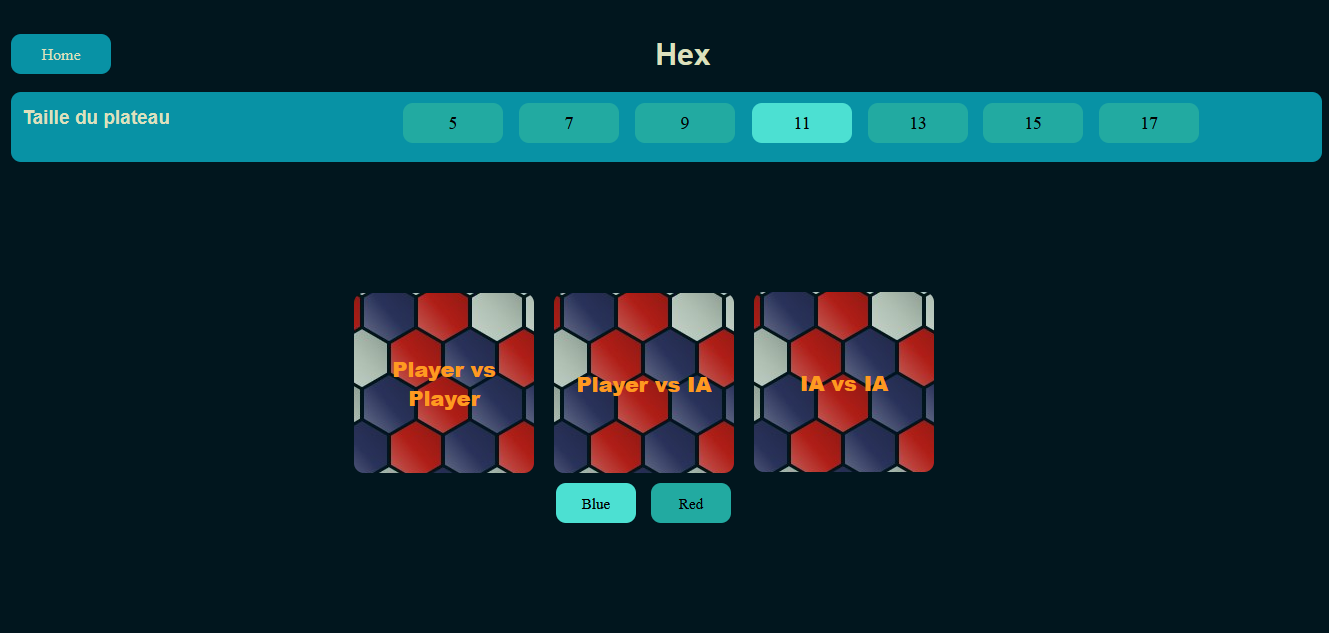
\includegraphics[width=\linewidth]{root/exemple_home}
        \caption{Page Home du Hex}\label{fig:exemple_home}
    \end{minipage}\hfill
    \begin{minipage}{0.33\textwidth}
        \centering
        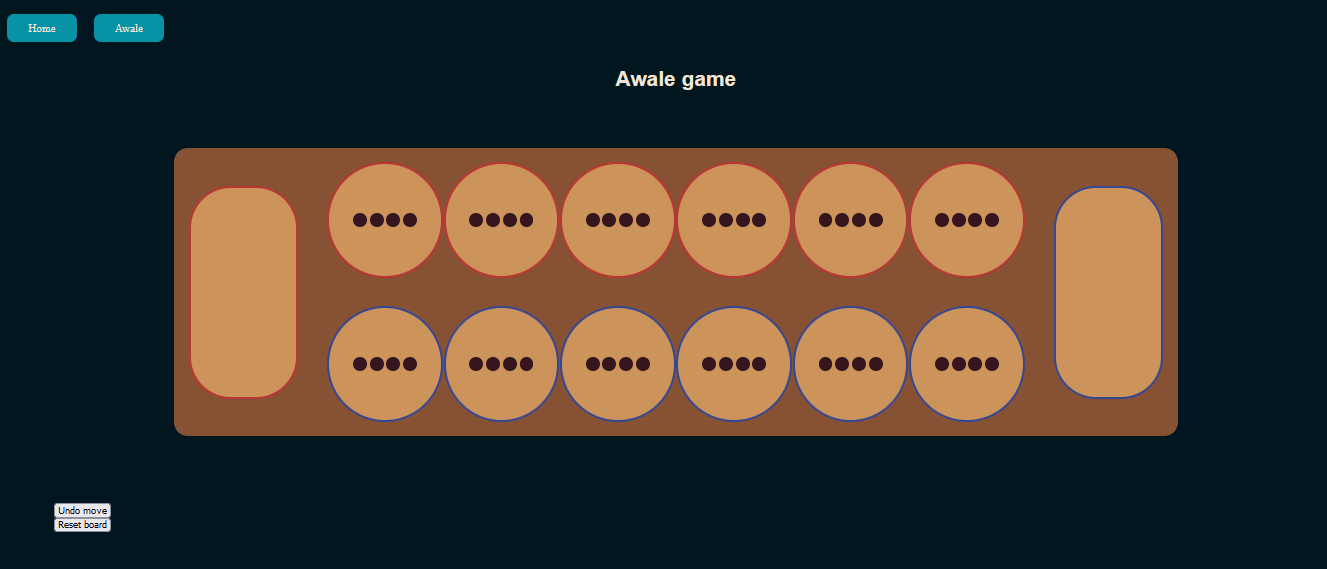
\includegraphics[width=\linewidth]{root/awale_board.png}
        \caption{Page initiale de jeu de l'Awalé}\label{fig:awale_board}
    \end{minipage}\hfill
    \begin{minipage}{0.33\textwidth}
        \centering
        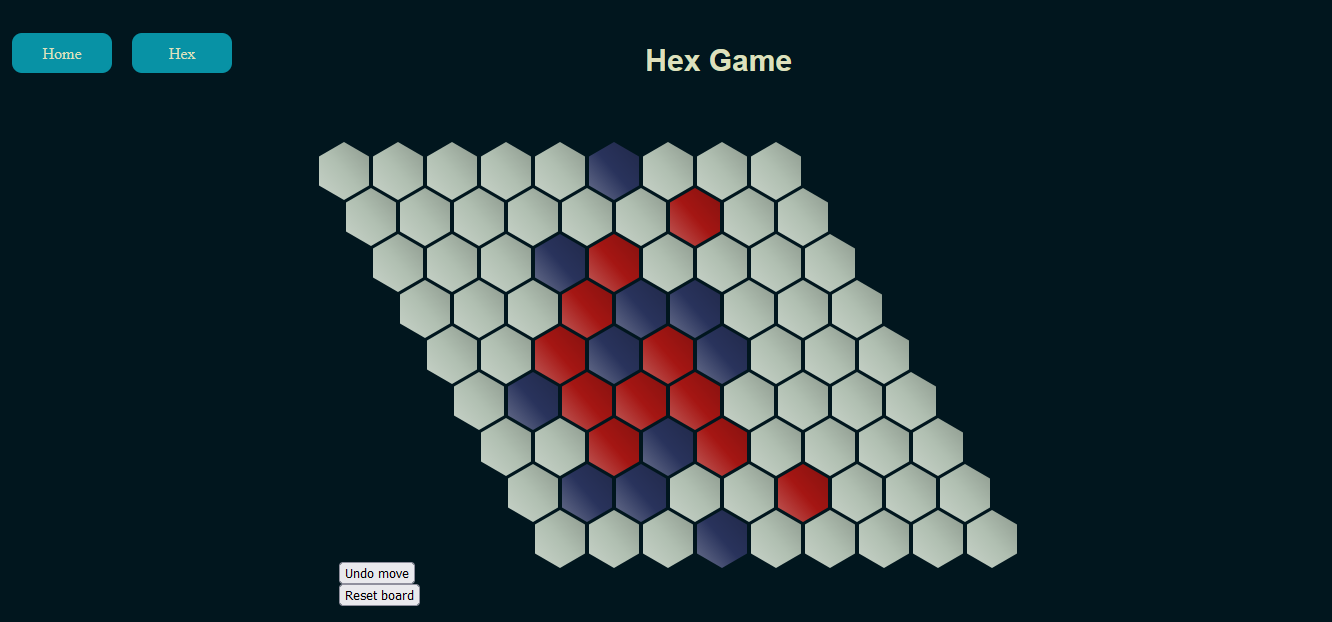
\includegraphics[width=\linewidth]{root/exemple_partie_hex}
        \caption{Exemple de partie de Hex en cours}\label{fig:hex_board}
    \end{minipage}
\end{figure}

% présenter les principales structures de données définies dans le cadre du
% projet. Décrire le format des données en entrée ou encore les conventions
% utilisées pour les entrées de vos programmes. Décrire les procédures de
% lecture et validation des entrées.
\subsubsection{Structures de données}
Les principales structures de données définies dans le cadre de ce projet sont les classes
\texttt{HexBoard} et \texttt{AwaleBoard}. Elles représentent respectivement les plateaux de jeu du Hex et de
l'Awalé. Ces classes contiennent les attributs et les méthodes nécessaires
pour représenter les plateaux de jeu et les joueurs. Elles permettent aussi d'effectuer les opérations de jeu
(placement de pions, déplacement de pions etc.) Les données sont fournies en entrée des programmes
sous la forme de chaînes de caractères qui représentent les paramètres de la partie (taille du
plateau, mode de jeu etc.) Les procédures de lecture et de validation
des entrées sont effectuées par les fonctions des modules Hex et Awalé qui vérifient que les
paramètres de la partie sont valides avant de commencer la partie.

% Statistiques : nombre de modules/composantes/classes/scripts développés.
% Nombre de lignes de code.
\subsubsection{Statistiques}
Voici quelques statistiques sur le logiciel développé dans le cadre de ce projet:
\begin{itemize}
    \item Nombre de modules (sans les tests): 39
    \item Nombre de classes: 11 (principalement dans les modules Hex et Awalé)
    \item Nombre de fonctions: 68 (en Python) et 99 (en JavaScript) pour 167 en tout
    \item Nombre de lignes de code: 1 405 (en Python), 2008 (en JavaScript), 553 (en HTML), 1 331 (en CSS)
    et 480 (en \LaTeX) pour un total de 5 777 lignes de code
\end{itemize}

\subsection{Intéractions entre les fichiers}
% Explication de l'interaction entre les fichiers pendant une partie
L'intéraction entre les fichiers de l'application est la même lors d'une partie de Hex ou 
d'Awalé. Le fichier \texttt{app.py} héberge l'application flask et gère l'intéraction entre le frontend et le 
backend pour les deux jeux.

\subsubsection{Initialisation de la partie}
La sélection du jeu et des paramètres de la partie se fait dans le fichier \texttt{home\_hex.html} pour le Hex
(respectivement \texttt{home\_awale.html} pour l'Awalé). Ces informations seront envoyées au fichier \texttt{app.py}
lorsqu'un clic souris sera effectué sur l'un des boutons. Le bouton sélectionné appellera dans le fichier \texttt{app.py} la 
fonction adéquate renvoyant la page HTML en prenant compte les choix effectués plus tôt. En parallèle, une instance du plateau de
jeu désiré sera créée dans le fichier \texttt{app.py}. 

\subsubsection{Déroulement d'une partie}
Lorsqu'une partie est jouée, l'information des pièces placées au Hex, ou des graines déplacées sur l'Awalé est récupérée par
le fichier JavaScript adapté: \texttt{game\_hexia.js} si la partie est une partie de Hex JcIA, ou encore 
\texttt{game\_awale.js} si la partie est une partie d'Awalé JcJ. Cette information est gérée par le capteur d'événements
\texttt{hex.onclick} pour le Hex et \texttt{pit.onclick} pour l'Awalé. Si un tel événement est entendu, le fichier JavaScript correspondant envoie une requête 
json au fichier \texttt{app.py} afin de savoir si le coup est valide. La validité du coup est gérée par une fonction appelée dans la classe du
plateau de jeu adéquat. Si le coup est valide, alors celui-ci est joué et rajouté à l'instance du plateau de jeu. Il est ensuite renvoyé au fichier 
JavaScript qui va s'occuper du nouvel affichage graphique (En modifiant le CSS ou le HTML). Si une erreur est attrapée, elle est renvoyée
au fichier JavaScript qui va afficher une alerte sur l'écran du joueur, indiquant la non-validité du coup. Lors du placement de chaque
hex (déplacement de graines pour l'Awalé), la fonction \texttt{check\_winner} de la classe du plateau est appelée afin de vérifier si un joueur a 
gagné. Si c'est le cas, alors la fonction questionnée par la requête json renvoie la variable \texttt{game\_over} égale à \texttt{True}. 
En récupérant cette variable, le fichier JavaScript va pouvoir procéder à une animation indiquant que la partie est terminée.
Nous détaillons l'affichage du chemin gagnant dans la section 4.



\subsection{Fonctions asynchrones}
L'envoi des différentes requêtes des fichiers JavaScript à \texttt{app.py} se fait grâce aux différents appels à la fonction \textit{fetch}.
La méthode globale \textit{fetch} démarre le chargement d'une ressource sur le réseau et retourne une promesse qui est résolue dès que la 
réponse est disponible. Cependant, le fait que la réponse ne soit renvoyée que lorsque celle-ci est disponible nous a gêné lors de l'implémentation
des modes JcIA et IAvIA pour les deux jeux. En effet, nous souhaitons que notre programme s'exécute de façon synchrone (ligne après ligne). 
Or, le \textit{fetch} peut prendre un certain temps avant de résoudre la promesse faite, cela est notamment dû à la lenteur des fonctions d'évaluation.
Ainsi, pour éviter que le reste du programme ne s'exécute avant la résolution de la promesse, nous avons décidé d'ajouter le décorateur 
\textsf{async} à notre fonction \textit{window.onload}. Ce simple décorateur nous a alors permis d'utiliser le mot-clé \textsf{await} devant les requêtes \textit{fetch}.
Celui-ci interrompt l'exécution de la fonction asynchrone et attend la résolution de la promesse passée. Ainsi, les requêtes se voient toujours résolues 
avant d'exécuter la suite du programme. Cela permet d'éviter que le joueur puisse jouer plusieurs coups pendant que l'IA « réfléchie », ou encore le fait
qu'une des deux IA dans le IAvIA joue plusieurs fois avant que l'autre ne joue.
